\subsection{Актуальные прикладные задачи и проблемы программной реализации их решений}

\begin{frame}

  \begin{itemize}
    \item Задачи математического моделирования.
    \item Задачи анализа данных.
    \item Задачи проектных инженерных расчётов.
    \item и~т.д.
  \end{itemize}

  \vspace{0.05\textheight}

  \begin{itemize}
    \item \textbf{Практически значимая программная реализация методов решений прикладных задач, как правило, является нетривиальной}
  \end{itemize}
\end{frame}

% --------------------------------------------------------------------------- %
\subsection{Программная реализация прикладных решений в команде}
% --------------------------------------------------------------------------- %
\begin{frame}

  \begin{itemize}
    \item Наличие в команде нескольких человек и распределение обязанностей по разработке отдельных этапов между ними положительно сказывается на качестве реализуемого ПО
  \end{itemize}

  \begin{figure}
    \begin{minipage}{0.49\textwidth}
      \centering
      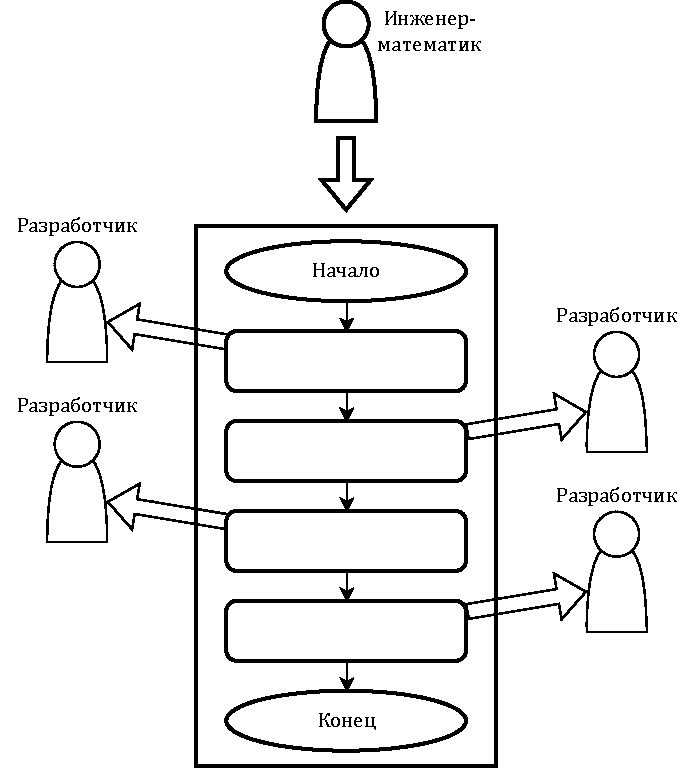
\includegraphics[height=0.6\textheight]{images/illustration.teamwork.pdf}
    \end{minipage}\hfill\begin{minipage}{0.49\textwidth}
      \begin{itemize}
        \item Введение новых разработчиков в проект влечёт за собой необходимость описывать для них логику реализуемого решения.
        \item Целесообразно включить разработку описания логики решения в процесс его программной реализации.
      \end{itemize}
    \end{minipage}\hfill
  \end{figure}

\end{frame}


% --------------------------------------------------------------------------- %
\subsection{Современные средства, направленные на упрощение реализации решений прикладных задач}
% --------------------------------------------------------------------------- %
\begin{frame}

  {\smaller[1]
    Среди современных средств упрощения разработки можно выделить следующие:
    \begin{itemize}
      \item научные системы управления потоком задач.
      \item платформы малокодовой разработки (LCPD).
    \end{itemize}
  }

  \begin{block}{Основной принцип}
    \smaller[1]
    Использование формальных описаний алгоритма решения при его непосредственной программной реализации.
  \end{block}

  \begin{figure}
    \begin{minipage}{0.49\textwidth}
      \centering
      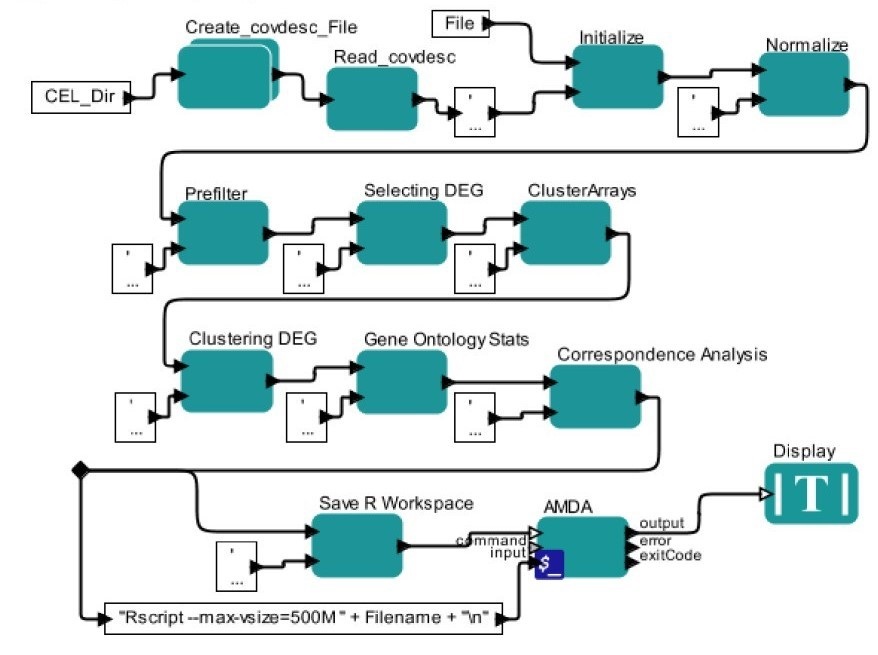
\includegraphics[width=\textwidth]{images/screenshot.KeplerWorkflow.jpg}
      \caption{\smaller[1] Пример описания алгоритма в научной системе управления потоком задач Kepler}
    \end{minipage}\hfill\begin{minipage}{0.49\textwidth}
      \centering
      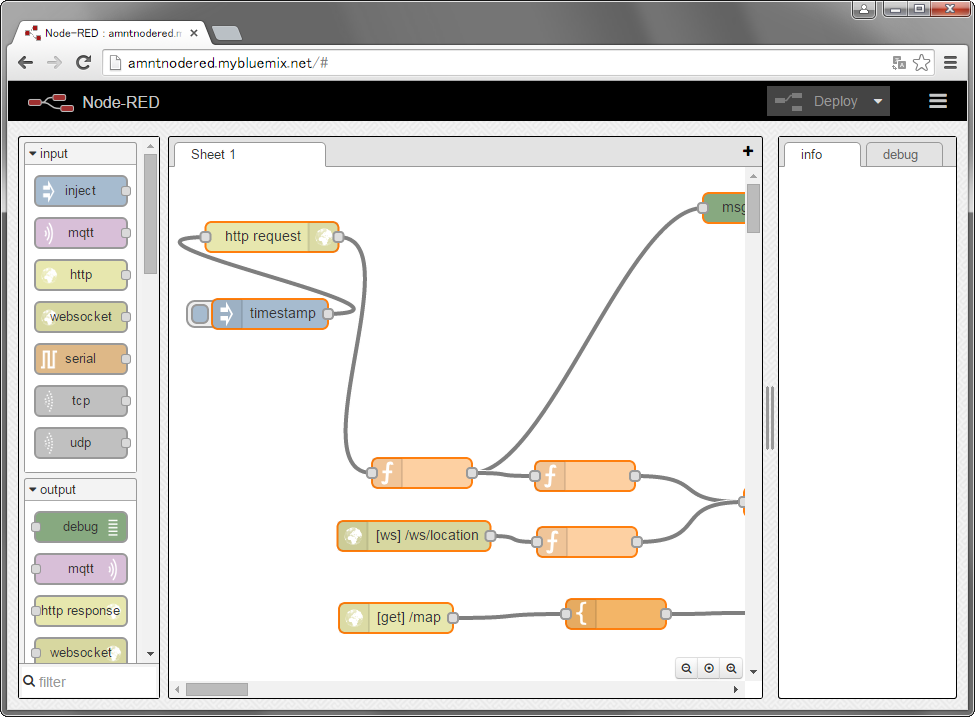
\includegraphics[width=\textwidth]{images/screenshot.NodeRED.png}
      \caption{\smaller[1] Пример описания алгоритма в LCPD Node-RED}
    \end{minipage}\hfill
  \end{figure}
\end{frame}

% --------------------------------------------------------------------------- %
\subsection{Подходы к построению формальному описанию логики процесса}
% --------------------------------------------------------------------------- %
\begin{frame}
  \begin{itemize}
    \item Можно выделить следующие подходы:
          \begin{itemize}
            \item Диаграммы потоков данных (DFD).
            \item Диаграммы потока управления.
            \item Диаграммы переходов состояний.
          \end{itemize}

    \item \textbf{Рассматриваемый в данной работе подход GBSE является частным случаем применения диаграмм переходов состояний.}
  \end{itemize}

\end{frame}



